\documentclass[twoside,11pt]{article}

\usepackage{blindtext}

% Any additional packages needed should be included after jmlr2e.
% Note that jmlr2e.sty includes epsfig, amssymb, natbib and graphicx,
% and defines many common macros, such as 'proof' and 'example'.
%
% It also sets the bibliographystyle to plainnat; for more information on
% natbib citation styles, see the natbib documentation, a copy of which
% is archived at http://www.jmlr.org/format/natbib.pdf

% Available options for package jmlr2e are:
%
%   - abbrvbib : use abbrvnat for the bibliography style
%   - nohyperref : do not load the hyperref package
%   - preprint : remove JMLR specific information from the template,
%         useful for example for posting to preprint servers.
%fhajkfhcuhfkahficdaui
% Example of using the package with custom options:
%
% \usepackage[abbrvbib, preprint]{jmlr2e}

\usepackage[preprint]{jmlr2e}
\usepackage{array}
\usepackage{longtable}
\usepackage{amsmath}
\usepackage{amssymb}


% Definitions of handy macros can go here

\newcommand{\dataset}{{\cal D}}
\newcommand{\fracpartial}[2]{\frac{\partial #1}{\partial  #2}}

% Heading arguments are {volume}{year}{pages}{date submitted}{date published}{paper id}{author-full-names}

% \usepackage{lastpage}
% \jmlrheading{23}{2022}{1-\pageref{LastPage}}{1/21; Revised 5/22}{9/22}{21-0000}{Author One and Author Two}

% Short headings should be running head and authors last names

\ShortHeadings{Optimizing Flight Departure Delay Predictions at Dubai Airport Using ML Techniques}{Alhosani, Alshamsi and Mohammed}
\firstpageno{1}

\begin{document}

\title{Optimizing Flight Departure Delay Predictions at Dubai Airport Using Machine Learning Techniques}

\author{\name Abdus Saboor Gaffari Mohammed \email b00105302@aus.edu \\
       \addr Department of Statistics\\
       University of Washington\\
       Seattle, WA 98195-4322, USA
       \AND
       \name Author Two \email two@cs.berkeley.edu \\
       \addr Division of Computer Science\\
       University of California\\
       Berkeley, CA 94720-1776, USA}

\author{\name Abdus Saboor Gaffari Mohammed \email b00105302@aus.edu \\
        \addr Department of Computer Science \& Engineering\\
        Master of Science in Machine Learning\\
        American University of Sharjah\\
        Sharjah, UAE
        \AND
        \name Khalifa Alshamsi \email b00078654@aus.edu \\
        \addr Department of Computer Science \& Engineering\\
        Master of Science in Machine Learning\\
        American University of Sharjah\\
        Sharjah, UAE
        \AND
        \name Latifa Alhosani \email g00104304@aus.edu \\
        \addr Department of Computer Science \& Engineering\\
        Master of Science in Machine Learning\\
        American University of Sharjah\\
        Sharjah, UAE
       }

\editor{My editor}

\maketitle

\begin{abstract}%   <- trailing '%' for backward compatibility of .sty file
Due to the rising demand for air travel, challenges have emerged in the handling of flight delays, which disadvantage customer satisfaction and operational effectiveness. The following project entails the use of supervised machine learning classification techniques to predict departure delays at Dubai Airport. In this model, weather information and other airport activities are integrated to categorize flights as “on time” or “delayed.” To do so, we will strive to outperform the current state-of-the-art results with the help of sophisticated machine learning approaches, hyperparameter tuning, novel preprocessing methods, and model ensembling. To mitigate the issue of data imbalance, the following oversampling approaches are employed. We will evaluate the performance of the system using performance metrics such as accuracy, precision, recall, and F1 score, with the goal of setting a new benchmark in departure flight delay prediction at Dubai Airport. 
\end{abstract}

\begin{keywords}
  flight delay prediction, supervised learning, machine learning
\end{keywords}

\section{Introduction}

The aviation industry has experienced exponential growth due to global population increases and technological advancements. According to the International Air Transport Association (IATA), the number of air passengers is projected to double by 2037, reaching approximately 8.2 billion annually (\citealp{usAirlineSawRecord}). While this growth drives economic benefits, it also poses significant challenges for the efficient management of air traffic. Among these, flight delays are particularly disruptive, as they compromise customer satisfaction and increase operational costs for airlines. 

Departure delays, influenced by local factors such as weather conditions and airport operations, present a specific challenge. In 2023, for instance, the average percentage of delayed departure flights in the U.S. reached 22.06\%, the highest level recorded in a decade (\citealp{bart2024}). The economic consequences are equally severe; in 2019 alone, delays led to losses of \$33 billion in the U.S., stemming from wasted fuel, extended labour costs, and passenger compensation (\citealp{aA2024}). These issues highlight the urgent need for accurate and effective predictive models to mitigate delays and enhance the efficiency of airport operations. 

Dubai Airport, as one of the busiest international transit hubs, provides a unique and complex environment for this study. Its high passenger volume, frequent connections, and regional weather patterns make it an ideal case for developing robust predictive models. Existing approaches to flight delay prediction often fall short in achieving sufficient accuracy or generalizability, underscoring the need for methodologies that surpass current state-of-the-art benchmarks. This gap in performance motivates the development of innovative solutions tailored to the specific operational characteristics of Dubai Airport. 

This project addresses these challenges by developing a supervised machine learning classification model to predict departure delays at Dubai Airport. The model integrates diverse data sources, including real-time weather data and airport operational metrics, to classify flights as either "on time" or "delayed." To enhance accuracy, advanced techniques such as hyperparameter tuning, model ensembling, and oversampling are employed. The system’s performance will be evaluated using metrics like accuracy, precision, recall, and F1 score. 

By addressing these challenges, this project aims to set a new benchmark for departure delay prediction. The anticipated outcomes include improved airport management strategies, enhanced passenger satisfaction, and reduced operational costs for airlines. These contributions will position the proposed system as a valuable tool for both researchers and industry practitioners seeking to address the persistent issue of flight delays. Moreover, the following sections will introduce the structure of this paper. Section 2 will explore the current state-of-the-art machine learning and deep learning approaches for prediction of departure flight delay and hightlight their contributions. Section 3, the methodology, will explain the proposed approach, including the integration of autoencoders for latent feature extraction, data preprocessing techniques, and the deployment of supervised machine learning models such as Feedforward Neural Networks and XGBoost. In Section 4, we will be evaluating the system’s performance using performance metrics such as accuracy, precision, recall, and F1 score, comparing it against current benchmarks. Lastly, Section 5 will conclude the study, summarizing key findings, discussing the implications for the aviation industry, and suggesting directions for future research.

\section{Related Works}
Accurately predicting flight delays has been a significant area of research, with various machine learning approaches demonstrating promising results. This section highlights three key studies that have contributed to the field, focusing on their methodologies, outcomes, and limitations.  

One of the methods that has gained huge interest and that is the use of state-of-the-art Recurrent Neural Networks (RNNs) like Long Short-Term Memory (LSTM) models. For Instance, \cite{liu2022flight} compared the performance of LSTM with traditional neural networks for departure flight delay prediction, with a greater focus on data integration and feature enhancement. The study combined flight-related attributes, such as time, airline, departure airport, and flight delay information, with weather data that included 124 features like monitoring location, time, temperature, cloud condition, air pressure, and wind speed. These datasets are sourced from the Bureau of Transportation Statistics (BTS) and the National Oceanic and Atmospheric Administration (NOAA) and merged to enhance prediction accuracy. After properly fusing two datasets, preprocessing steps included data cleaning, such as removing outliers and deleting features with more than 80\% missing values as well as records that lack sufficient variables across multiple features. This reduced the dataset from an initial size of 5,819,079 records to 105,071 records with 35 features. Afterward, numerical features were standardized using Min-Max normalization, while all categorical features were encoded using label encoding to avoid the dimensionality expansion caused by one-hot encoding. The authors configured a three-layer LSTM network with 128 hidden units, a learning rate of 0.01, a batch size of 128, six epochs, and cross-entropy as the loss function. Consequently, the proposed method achieved accuracy of 94.8\%, significantly outperforming multi-layer perception (MLP) and support vector machine (SVM).  

Though LSTM models have shown its capability to handle temporal dependencies, recent developments have focused on hybrid deep learning models to improve spatial and temporal feature extraction. For example, \cite{qu2023flight} proposed a novel hybrid deep learning method, SimAM-CNN-MLSTM, for classifying departure flight delay propagation. The method combines the strengths of Convolutional Neural Networks (CNN) for spatial feature extraction and Mogrifier Long Short-Term Memory (MLSTM) for processing temporal dependencies combined with the Simple Attention Module (SimAM) for prioritizing key features and refining spatial-temporal relationships without adding extra computational overhead. The study utilized a dataset of 1,048,576 flight records from March 2018 to May 2019 provided by the Civil Aviation Administration of China (ECRA) that contain mostly flight attributes such as flight path, cruise altitude and speed. After preprocessing steps, such as removing outliers and null entries, the dataset was reduced to 36,287 flight chains. Afterwards, Min-Max normalization was applied to standardize numerical features, while categorical features were encoded using the CatBoost algorithm to prevent the expansion of features typically caused by one-hot encoding. The proposed architecture includes a 1×1 convolution layer for dimensionality reduction, a 3×3 convolution kernel for spatial feature extraction, and then SimAM for dynamically assigning importance to relevant neurons while suppressing irrelevant ones. These blocks are repeated three times and then connected to an MLSTM cell which enables interaction between the previous state and current input for effective temporal modeling. As a result, SimAM-CNN-MLSTM model achieved accuracy, precision, recall and F1 score of 91.3\%, 82.5\%, 87.4\%, and 84.9\%, respectively and outperforming other several techniques such as standalone LSTM, C4.5 Decision tree, CBAMCondenseNet and ATD Bayesian network.  

Besides the advanced deep learning architectures, tree-based ensemble methods are also found to be useful for flight delay prediction. A study by \cite{tao2021flight} leveraged the strengths of the Light Gradient-Boosting Machine (LightGBM) algorithm with optimized parameters to predict departure flight delays using regression and to compare its performance against other tree-based models. The dataset is provided by Atlanta Hartsfield-Jackson International Airport (ATL) for flight data in 2018, and it was cleaned by filling null feature entries with their mean values, while small samples with missing values were removed. The dataset includes 15 different airlines, and statistics show that departure flight delays are more frequent among low-cost airlines compared to others; thus, the airline company feature is considered as ordinal categorical variables and encoded using label encoding. As for feature selection, it was performed automatically by the built-in embedding method of LightGBM and eliminates features with a weight coefficient below a specified threshold of feature importance, while retaining the most relevant features. Interestingly, the arrival time of taxis at departure and destination airports was found to influence the model’s predictions. Ultimately, the results demonstrated that LightGBM with optimized parameters through grid search achieved a Mean Absolute Error (MAE) of 4.57 minutes with a training time of just 0.133 seconds, representing at least a 16\% improvement in accuracy and a 26-fold increase in training speed compared to Gradient Boosted Decision Trees (GBDT) and eXtreme Gradient Boosting (XGBoost). The experimental results highlight LightGBM’s superiority compared to others as it offers faster training speeds due to its parallel learning capabilities, lower memory consumption, and overall better performance. 

In another study, \cite{hatipoglu2024predictive} conducted a comprehensive evaluation of supervised machine learning models to address the challenge of data imbalance in departure flight delay classification using the Synthetic Minority Over-Sampling Technique (SMOTE). The authors highlighted that data imbalance can artificially inflated accuracy metric since models often tend to favor the majority class. Thus, SMOTE was employed to generate synthetic samples for the minority class and increase their instances to match that of the majority class, ensuring the prevention of bias. The study utilized 40,077 flight records (21\% minority) from a Turkish airport spanning 2016 to 2018 and combined with open-source weather data obtained from the rp5.ru website. Preprocessing steps involved applying SMOTE and encoding all categorical variables using one-hot encoding. Afterwards, models including Neural Networks, Random Forest, Logistic Regression, Naïve Bayes, CatBoost, LightGBM, and XGBoost were trained with Bayesian optimization for fast and efficient hyperparameter tuning. To enhance interpretability and reduce dimensionality, SHAP (SHapley Additive exPlanations) was employed to disregard irrelevant features while keeping important features. Results showed that SMOTE significantly improved the F1 score and recall for all models, and XGBoost achieved the best overall performance.

Furthermore, studies have shown the importance of using a variety of parameters or data sources to improve the accuracy of flight delay predictions. For instance, \cite{integratingMultipleData} combined a variety of data such as airport information, operational data, geographic data, and weather conditions to predict flight delays using explainable machine learning techniques. Their work shown the impact of linear discriminant analysis for recognizing the attributes that contribute to flight delays such as wind speed and international flight status. As shown in Table 1, the study used an intensive dataset which contained attributes such as flight type, destination airport elevation, and weather metrics like wind speed and air pressure.  

\section{Methodology}
\subsection{Dataset}
The flight and departure details at Dubai airport were sourced from open access API provided by \cite{dubaiairportsDatasetDa_flight_information_departuresopenapi} on the dubaipulse \footnote{www.dubaipulse.com} platform. The data queried from the API contains details like the scheduled offblock time, actual offblock time, Airline, flight number, destination, airplane model, etc. The details about all the API fields are given in Table \ref{tbl:apiFields}. Using the API we were able to fetch the flight records from March 2020 to October 2024. Although the timeframe is large, more than 4 years, not all the records had all the required details, therefore we opted to only consider those records that had both the scheduled and actual offblock time. Figure \ref{fig:flightsYearMonth} shows the number of flights that had correct data per year/month, from which we can gather that the data is no longer being maintained. 
In addition to the flight data, the historical weather details at the time of the flights were also collected. The weather data used is the United Arab Emirates ASOS data recorded at the OMDB station at Dubai Airport, which is made available on Iowa State University's Environmental Mesonet website \footnote{https://mesonet.agron.iastate.edu}. The data collected contains details like the temparature, humidity, wind direction, coluds, rain and other weather conditions. Table \ref{tbl:weatherFields} shows all the fields available and their descriptions. 
\begin{figure}
  \centering
  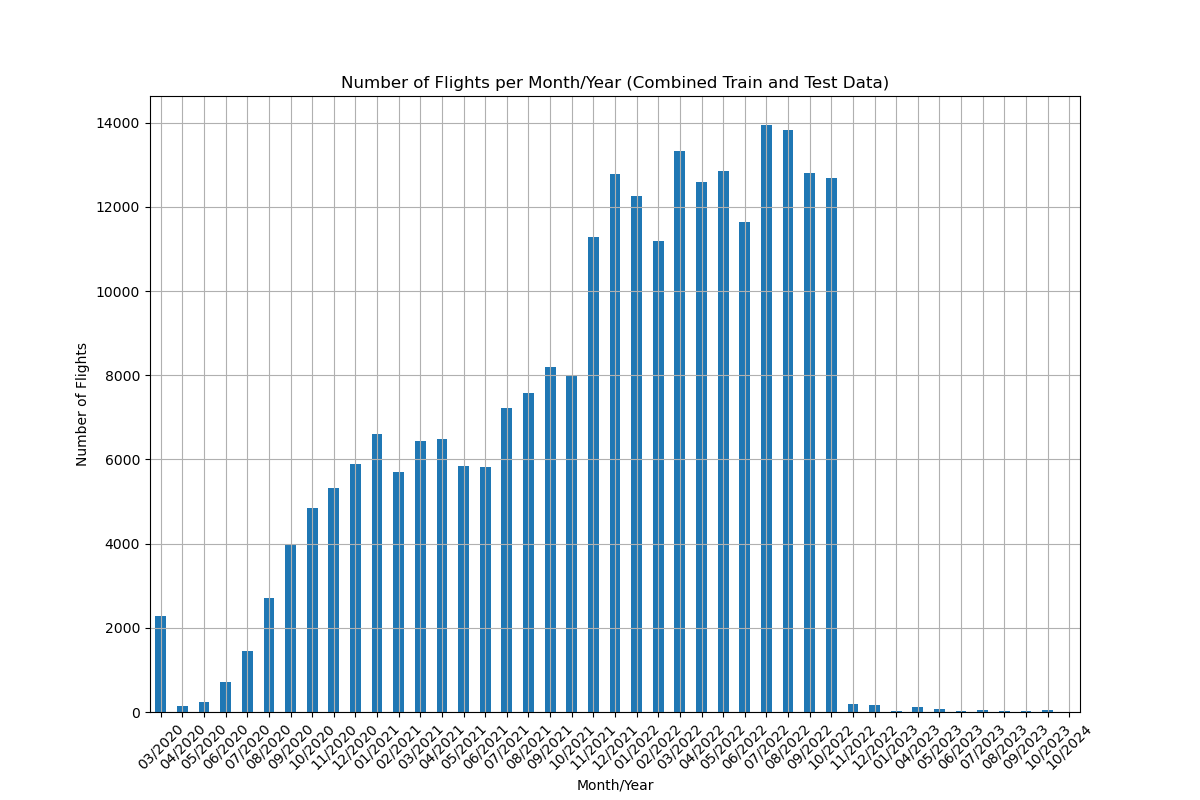
\includegraphics[width=0.85\textwidth]{images/flights_per_month_year.png}
  \caption{Number of records per month/year that had valid data for scheduled and actual time}
  \label{fig:flightsYearMonth}
\end{figure}
\subsubsection{Combining data}
For the task of prediction by machine learning we prefer data that is be combined into one, therefore the two datasets containing the flight and weather details were combinded based on the flight's scheduled time. The weather data collected contains only hourly recording, so in order to match them with the flights' scheduled time, the scheduled times were first rounded off to nearest hour and then the two datasets were joined on the rounded off scheduled time and the time of weather reading. If weather readings at the time any flight are missing then the last available hour's readings were used. Similarly if any of the features were missing from the weather data then the last available data was used, like for wind direction.

\subsection{Proposed Approach}
The proposed model for flight delay prediction is a hybrid model that combines unsupervised and supervised learning. The approach employs an autoencoder for feature extraction through unsupervised learning and later trains or finetune other downstream machine learning models using the extracted features in a supervised manner. The full working of the proposed model is depicted in Figure \ref{fig:model}. During the training phase the training data is fed to the encoder which generates the latent feature, these latent features are fed to the decoder to reconstruct the input data (\citealp{hintonReducingDimensionalityData2006}), the loss function used is the reconstruction MSE given as Eq. \ref{eq:mse_recon}. 
\begin{equation}
  \label{eq:mse_recon}
  MSE_{Autoencoder} = \frac{1}{n} \sum_{i=1}^{n} ||x_i - \hat{x_i}||^2
\end{equation}
\begin{figure}
  \centering
  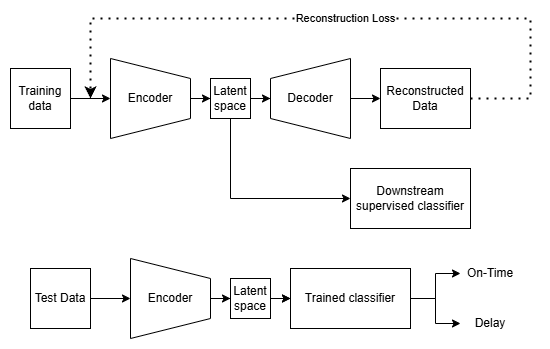
\includegraphics[width=0.85\textwidth]{images/model.png}
  \caption{Working of the proposed model}
  \label{fig:model}
\end{figure}
After the autoencoder is trained, the latent features generated by the encoder are then used to train the downstream supervised classifier. During the testing phase the test data is first fed to the encoder to extract the latent features, which are fed to the downstream trained models for the classification task.

The use of autoencoder allows us to reduce the dimension of the data by compressing it to its latent features. Reducing the dimensionality helps to to mitigate the curse of dimensionality and reduce the computational cost. An autoencoder is capable of learning the non-linear relationships and patterns of complex data effectively making them preferable over other traditional dimensionality reduction techniques. The latent features generated by autoencoder contain more information and less noise when compared to the raw features, allowing them to be used to improve the performance of supervised classifiers. Another benefit of using the latent features is that the can reduce the risk of overfitting, due to the reduced input dimension and more meaningful representation (\citealp{berahmandAutoencodersTheirApplications2024}). Another benefit of using the latent features produced by autoencoders is that they tend learn representations that are better generalizable (\citealp{gabdullinLatentSpaceConfiguration2024}), reduce the correlation among features and deal with any redundancy in the data.

\subsection{Data Preprocessing}
Before the data is used to train the model, it needs to be preprocessed to make it cleaner and interpretable by the model. The flight data collected from the API did not contain any feature that represented if the flight is delay or not, therefore a new feature was created for the same. According to FAA, a flight is considered as delayed if it is delayed by more than 15mins from the scheduled time, taking that as a base we have marked a flight as delayed if the difference between the \emph{scheduledoffblocktime} and \emph{actualoffblocktime} is more than 15 mins.
\[
  d^i = t_{aot}^i - t_{sot}^i
  \]

\[
  s^i = \begin{cases}
      \text{Delay}, & \text{when } d^i\geq 15\\
      \text{On-Time}, & \text{otherwise }
      \end{cases}
\]

Many features from the weather dataset that were all empty or 0 were dropped, like snow and snow level as there is no snow in the UAE. Any missing readings in the weather data were filled with values from the immediately previous reading. In case of few features, where there are no incidents or weather anomalies the readings are not mentioned, i.e. in normal conditions they are left empty. These features were imputed with a default values. In for any categorical column with missing values, they filled with default values as well. Any feature that had high correlation with other feature were dropped along with features that were just Arabic versions of existing English columns. As we have already extracted the delay feature, we can drop all date related features and only keep the \emph{scheduledoffblocktime}. 

After all the missing values are imputed and features dropped we need to encode the features into numerical values so that they can be fed to the autoencoder. To do this, , the \emph{scheduledoffblocktime} is broken into its individual components - day of month, day of week, month of year, hour of day and minutes of hour, and as all the categorical features are nominal they were all one-hot encoded. After encoding the features were standardized to have zero mean and standard deviation of one.

\section{Experiment and Results}
In this section, we evaluate the performance of the model using standard metrics such as accuracy, precision, recall, and F1-score. The formulas for these metrics are as follows:

\begin{description}
    \item[Accuracy] Measures the proportion of correctly predicted instances out of the total observations. It reflects the overall effectiveness of the model but may be misleading in cases of imbalanced datasets.
        % Accuracy Formula
        $$
        {Accuracy} = \frac{{TP} + {TN}}{{TP} + {TN} + {FP} + {FN}}
        $$
    \item[Precision] Measures the proportion of correctly predicted positive instances out of all instances predicted as positive. In this context, it indicates the fraction of flights predicted to be delayed that are actually delayed.
        % Precision Formula
        $$
        {Precision} = \frac{{TP}}{{TP} + {FP}}
        $$
    \item[Recall] Measures the proportion of actual positive instances that were correctly identified by the model. It indicates the fraction of truly delayed flights that were predicted as delayed.
        % Recall Formula
        $$
        {Recall} = \frac{{TP}}{{TP} + {FN}}
        $$  
    \item[F1 Score] Combines precision and recall into a single metric by calculating their harmonic mean. It provides a balanced evaluation of the model’s performance.
        % F1-Score Formula
        $$
        {F1 Score} = 2 \times \frac{{Precision} \times {Recall}}{{Precision} + {Recall}}
        $$
\end{description} 

\section{Limitations and Future work}

\section{Conclusion}



\acks{}

\appendix

\section{Dataset Details}

% \begin{longtable}{>{\hspace{0pt}}m{0.192\linewidth}>{\hspace{0pt}}m{0.552\linewidth}>{\hspace{0pt}}m{0.09\linewidth}>{\hspace{0pt}}m{0.092\linewidth}}
% \label{api_fields}
% \caption{Details of data fields returned by the Dubai Airport departure flights API}\\
% bf{Name}           & bf{Description}                                                                & bf{Data type} & bf{ Language }  \endfirsthead 
% \hline\hline
% aodbuniquefield         & Unique identifier for the flight (Primary Key)                                      & number             & English              \\ 
% \hline
% estimatedoffblocktime   & Estimated Departure time
%   of a flight from~DXB                                     & datetime           & English              \\ 
% \hline
% scheduledoffblocktime   & Scheduled departure time of a flight from DXB                                       & datetime           & English              \\ 
% \hline
% publicscheduleddatetime & The scheduled departures
%   time of a departing~flight that is made public           & datetime           & English              \\ 
% \hline
% actualtakeofftime       & The time when aircraft
%   departed fom the runway                                    & datetime           & English              \\ 
% \hline
% actualoffblocktime      & The time when the
%   aircraft was pushed back~from the stand~                        & datetime           & English              \\ 
% \hline
% aircraftparkingposition & The name of the stand the aircraft is parked                                        & string             & English              \\ 
% \hline
% publicgatenumber        & Gate number from where
%   the passenger will board~the flight                        & string             & English              \\ 
% \hline
% checkinallocationfrom   & Check in counter                                                                    & string             & English              \\ 
% \hline
% checkinallocationto     & Check in counter                                                                    & string             & English              \\ 
% \hline
% airlinename             & Name of the airline which
%   is the operating the flight                             & string             & English              \\ 
% \hline
% airlinenamea            & Name of the airline which
%   is operating the flight~in Arabic                       & string             & Arabic               \\ 
% \hline
% vianame                 & City Name of the Via                                                                & string             & English              \\ 
% \hline
% vianamea                & City Name of the Via in
%   Arabic                                                    & string             & Arabic               \\ 
% \hline
% destinationname         & City Name of the destination                                                        & string             & English              \\ 
% \hline
% destinationnamea        & City Name of the Last
%   destination in Arabic                                       & string             & Arabic               \\ 
% \hline
% flightstatus            & Status description of the
%   flight eg.: Arrived, Landed, Boarding, Final Call, etc. & string             & English              \\ 
% \hline
% flightstatustexta       & Flight status description
%   in Arabic                                               & string             & Arabic               \\ 
% \hline
% flightnumber            & Alphanumeric Flight
%   number - Airline IATA Code +~Number eg.: AA123                & string             & English              \\ 
% \hline
% jointflightnumber       & All flight Numbers
%   related to the~main flight, eg: B6 5061                        & string             & English              \\ 
% \hline
% traffictype             & Traffic type description of the flight                                              & string             & English              \\ 
% \hline
% aircraftterminal        & Terminal from which the flight is operating                                         & string             & English              \\ 
% \hline
% aircraftregistration    & Alphanumeric identifier for the flight eg
%   :A6ALI                                  & string             & English              \\ 
% \hline
% traffictypecode         & Traffic type code of the
%   flight eg.: Passenger/Cargo etc.                         & string             & English              \\ 
% \hline
% arrivalordeparture      & Arrival or Departure Identifier A/D                                                 & string             & English              \\ 
% \hline
% lastchanged             & Last updated time                                                                   & datetime           & English              \\ 
% \hline
% airlinecode\_iata       & Two letter code for the
%   Airline which operates the flight, eg.: EK                & string             & English              \\ 
% \hline
% airlinecode\_icao       & Three letter code for the
%   Airline which~~~operates the flight, eg.: UAE           & string             & English              \\ 
% \hline
% destination\_iata       & IATA three letter code
%   for the destination airport, eg: SYD                       & string             & English              \\ 
% \hline
% destination\_icao       & ICAO four letter code for the destination
%   airport                                 & string             & English              \\ 
% \hline
% via\_iata               & IATA three letter code for the via(route)
%   airport                                 & string             & English              \\ 
% \hline
% via\_icao               & ICAO three letter code for the via(route)
%   airport                                 & string             & English              \\ 
% \hline
% aircraft\_iata          & IATA sub category code of
%   the operating flight                                    & string             & English              \\ 
% \hline
% aircraft\_icao          & ICAO main category code of the operating flight                                     & string             & English              \\ 
% \hline
% flightstatuscode        & Flight status code                                                                  & string             & English             
% \end{longtable}


\bibliography{references}

\end{document}
